\documentclass[dutch]{ucll-slides}
\usepackage{pxfonts}
\usepackage{tikz}
\usepackage{calc}
\usepackage{ucll-code}
\usepackage{hyperref}


\usetikzlibrary{calc,shadows,tikzmark,shapes.multipart,arrows.meta}

\coursename{Scripttalen}
\title{IO}


\tikzset{
  file/.style={draw,fill=green!50,drop shadow,minimum width=3cm,minimum height=1cm},
  process/.style={draw,fill=blue!50,drop shadow,minimum width=3cm,minimum height=1cm},
  datum/.style={draw,fill=red!50,minimum width=.5cm,minimum height=.5cm,font=\tiny\ttfamily},
  stream/.style={ultra thick,-latex}
}

\begin{document}

\maketitle

\section{Input Streams}

\frame{\tableofcontents[currentsection]}

\begin{frame}
  \frametitle{Bestand Inlezen}
  \begin{itemize}
    \item Bestand is opeenvolging van bytes
    \item We kunnen bestand byte per byte uitlezen
  \end{itemize}
  \code[language=python]{readable-file.py}
\end{frame}

\begin{frame}
  \frametitle{Netwerkdata Ontvangen}
  \begin{itemize}
    \item Via een netwerkconnectie ontvangen we data
    \item Deze data is een reeks van bytes
    \item We kunnen deze bytes om beurt opvragen
  \end{itemize}
  \code[language=python]{readable-network.py}
\end{frame}

\begin{frame}
  \frametitle{Toetsenbordinvoer}
  \begin{itemize}
    \item Elke toetsaanslag genereert data
    \item We kunnen deze data opvragen
  \end{itemize}
  \code[language=python]{readable-keyboard.py}
\end{frame}

\begin{frame}
  \frametitle{Patroon}
  \begin{itemize}
    \item Drie klassen met methodes
          \begin{itemize}
            \item \texttt{read\_byte} op \texttt{FileReader}
            \item \texttt{receive\_byte} op \texttt{NetworkDataReceiver}
            \item \texttt{wait\_for\_input} op \texttt{KeyboardInput}
          \end{itemize}
    \item Lijken veel op elkaar
    \item Telkens methode om byte op te vragen
  \end{itemize}
\end{frame}

\begin{frame}
  \frametitle{Abstraheren tot Input Stream}
  \begin{itemize}
    \item Bron (bestand/netwerk/toetsenbord) maakt niet uit
    \item Bytes kunnen uitlezen is belangrijkst
    \item We kunnen de bronnen abstraheren tot ``bytegenerators''
  \end{itemize}
  \begin{center}
    \begin{tikzpicture}
      \node[rotate=90,file] at (-1,0) {%
        \only<1>{bestand}%
        \only<2>{netwerk}%
        \only<3>{toetsenbord}%
        \only<4>{muis}%
        \only<5>{micro}%
        \only<6>{scanner}%
        \only<7>{kinect}%
      };

      \foreach[count=\i] \b in {41, F1, 90, AD, 19} {
        \node[draw,minimum size=0.75cm,drop shadow,fill=red!50] at (\i, 0) {\b};
      }
      \node at (6,0) {\tiny\dots};

      \draw[ultra thick,-latex] (1,-1) -- (6,-1) node[below,midway] {\ttfamily get\_next\_byte()};

      \node[rotate=-90,process] at (8,0) {programma};
    \end{tikzpicture}
  \end{center}
\end{frame}

\begin{frame}
  \frametitle{Voordelen}
  \code[language=python,font=\small,width=.9\linewidth]{abstract-reading.py}
  \begin{itemize}
    \item \texttt{process\_input} kan werken met alle drie types input
    \item Enige voorwaarde: \texttt{stream} heeft \texttt{get\_next\_byte()}
  \end{itemize}
\end{frame}

\begin{frame}
  \frametitle{Voorbeeld}
  \begin{center}
    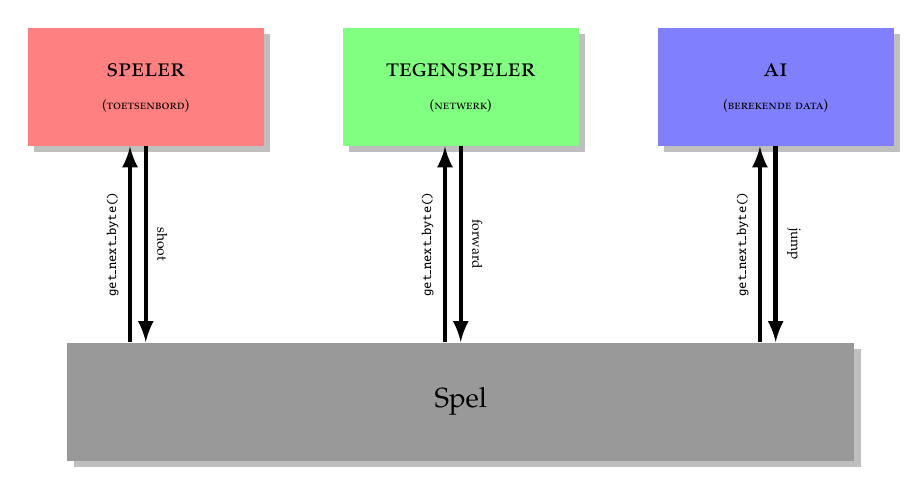
\begin{tikzpicture}[player/.style={minimum width=3cm,minimum height=1.5cm,drop shadow,font=\scshape},
                        local human player/.style={player,fill=red!50},
                        remote human player/.style={player,fill=green!50},
                        ai player/.style={player,fill=blue!50},
                        game/.style={drop shadow,fill=black!40,minimum width=10cm,minimum height=1.5cm},
                        communication/.style={ultra thick,-latex}]
      \node[local human player] (local) at (-4,0) {
        \begin{tabular}{c}
          speler \\
          \tiny (toetsenbord)
        \end{tabular}
      };
      \node[remote human player] (remote) at (0,0) {
        \begin{tabular}{c}
          tegenspeler \\
          \tiny (netwerk)
        \end{tabular}
      };
      \node[ai player] (ai) at (4,0) {
        \begin{tabular}{c}
          ai \\
          \tiny (berekende data)
        \end{tabular}
      };

      \node[game] (game) at (0,-4) {Spel};

      \draw[communication] let \p1=(local.south), \p2=(game.north) in
                           ($ (\x1,\y2) + (-0.2,0) $) -- ($ (\x1,\y1) + (-0.2,0) $)
                           node[midway,above,font=\tiny\ttfamily,sloped] {get\_next\_byte()};

      \draw[communication] let \p1=(local.south), \p2=(game.north) in (\x1,\y1) -- (\x1,\y2)
                           node[midway,above,font=\tiny,sloped] {shoot};

      \draw[communication] let \p1=(remote.south), \p2=(game.north) in
                           ($ (\x1,\y2) + (-0.2,0) $) -- ($ (\x1,\y1) + (-0.2,0) $)
                           node[midway,above,font=\tiny\ttfamily,sloped] {get\_next\_byte()};

      \draw[communication] let \p1=(remote.south), \p2=(game.north) in (\x1,\y1) -- (\x1,\y2)
                           node[midway,above,font=\tiny,sloped] {forward};

      \draw[communication] let \p1=(ai.south), \p2=(game.north) in
                           ($ (\x1,\y2) + (-0.2,0) $) -- ($ (\x1,\y1) + (-0.2,0) $)
                           node[midway,above,font=\tiny\ttfamily,sloped] {get\_next\_byte()};

      \draw[communication] let \p1=(ai.south), \p2=(game.north) in (ai) -- (\x1,\y2)
                           node[midway,above,font=\tiny,sloped] {jump};
    \end{tikzpicture}
  \end{center}
  \begin{itemize}
    \item Spel enkel ge\"interesseerd in data, bron maakt niets uit
  \end{itemize}
\end{frame}

%%% Local Variables:
%%% mode: latex
%%% TeX-master: "io"
%%% End:

\section{Output Streams}

\frame{\tableofcontents[currentsection]}

\begin{frame}
  \frametitle{Naar Bestand Schrijven}
  \begin{itemize}
    \item Bestand is in feite lijst van bytes
    \item We kunnen bytes toevoegen aan deze lijst
  \end{itemize}
  \code[language=python]{writable-file.py}
\end{frame}

\begin{frame}
  \frametitle{Netwerkdata Sturen}
  \begin{itemize}
    \item Via een netwerkconnectie sturen we data
    \item Deze data is een reeks van bytes
    \item We kunnen deze bytes na elkaar versturen
  \end{itemize}
  \code[language=python]{writable-network.py}
\end{frame}

\begin{frame}
  \frametitle{Abstraheren tot Output Stream}
  \begin{itemize}
    \item Ontvanger (bestand/netwerk) maakt niet uit
    \item Bytes kunnen schrijven is belangrijkst
    \item Abstractie ``byte ontvangers''
  \end{itemize}
  \begin{center}
    \begin{tikzpicture}
      \node[rotate=90,file] at (-1,0) {%
        \only<1>{bestand}%
        \only<2>{netwerk}%
        \only<3>{speakers}%
        \only<4>{scherm}%
      };

      \foreach[count=\i] \b in {41, F1, 90, AD, 19} {
        \node[draw,minimum size=0.75cm,drop shadow,fill=red!50] at (\i, 0) {\b};
      }
      \node at (6,0) {\tiny\dots};

      \draw[ultra thick,latex-] (1,-1) -- (6,-1) node[below,midway] {\ttfamily write\_byte()};

      \node[rotate=-90,process] at (8,0) {programma};
    \end{tikzpicture}
  \end{center}
\end{frame}

\begin{frame}
  \frametitle{Streams zijn niet Python-specifiek}
  \begin{itemize}
    \item Java: \link{https://docs.oracle.com/javase/7/docs/api/java/io/InputStream.html}{InputStream}, 
          \link{http://docs.oracle.com/javase/7/docs/api/java/io/OutputStream.html}{OutputStream},
          \link{https://docs.oracle.com/javase/7/docs/api/java/nio/channels/Channel.html}{channels}
    \item C++: \link{http://www.cplusplus.com/reference/iostream/}{iostream header file}
    \item Python: \link{https://docs.python.org/3/library/io.html}{io module}
    \item Ruby: \link{http://ruby-doc.org/core-2.0.0/IO.html}{IO klasse}
    \item C$^\sharp$: \link{https://msdn.microsoft.com/en-us/library/system.io.stream(v=vs.110).aspx}{Stream klasse}
  \end{itemize}
\end{frame}

%%% Local Variables:
%%% mode: latex
%%% TeX-master: "io"
%%% End:

\section{Pipelines}

\frame{\tableofcontents[currentsection]}

\begin{frame}
  \frametitle{Voorbeeld: Code}
  \code[language=python3]{processes.py}
  \begin{itemize}
    \item \texttt{increment} leest ints, incrementeert ze, en schrijft ze weg
    \item \texttt{double} leest ints, verdubbelt ze, en schrijft ze weg
  \end{itemize}
\end{frame}

\begin{frame}
  \frametitle{Voorbeeld: Visualisatie}
  \begin{center}
    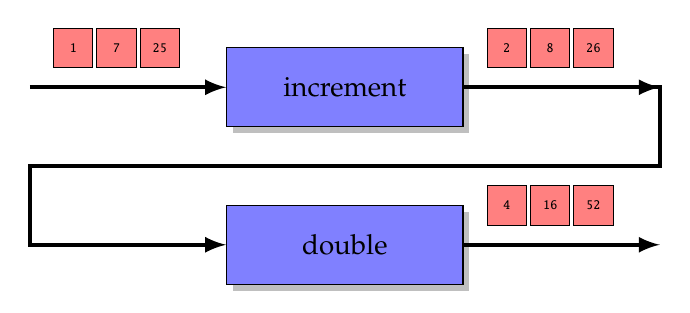
\begin{tikzpicture}
      \node[process] (increment) at (0,1) {increment};
      \node[process] (double) at (0,-1) {double};

      \draw[stream] (-4,1) -- (increment.west);
      \foreach[count=\i,evaluate={\i*0.55-4} as \j] \x in {1, 7, 25} {
        \node[datum] at (\j,1.5) {\x};
      }

      \visible<2>{
        \draw[stream] (increment.east) -- (4,1);
      }

      \visible<2->{
        \foreach[count=\i,evaluate={\i*0.55} as \j] \x in {2, 8, 26} {
          \node[datum] at ($ (increment.east) + (\j,0.5) $) {\x};
        }
      }

      \visible<3->{
        \draw[stream] (increment.east) -- (4,1) -- (4,0) -- (-4,0) -- (-4,-1) -- (double.west);
      }

      \visible<4>{
        \foreach[count=\i,evaluate={\i*0.55} as \j] \x in {4, 16, 52} {
          \node[datum] at ($ (double.east) + (\j,0.5) $) {\x};
        }
        \draw[stream] (double.east) -- (4,-1);
      }
    \end{tikzpicture}
  \end{center}
\end{frame}

\begin{frame}
  \frametitle{Pipelines}
  \begin{itemize}
    \item Output kan verbonden worden met andermans input
    \item Ketting opbouwen van ``processors''
    \item Ketting heet \emph{pipeline}
  \end{itemize}
  \vskip5mm
  \structure{Vb: Downloaden, Comprimeren, Encrypteren en Bewaren}
  \begin{center}
    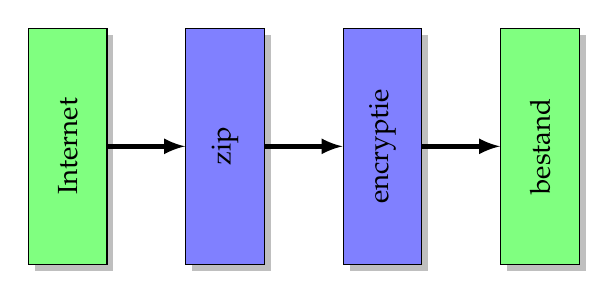
\begin{tikzpicture}[rotate=90,transform shape]
      \node[file] (input) at (0,6) {Internet};
      \node[process] (process 1) at (0,4) {zip};
      \node[process] (process 2) at (0,2) {encryptie};
      \node[file] (output) at (0,0) {bestand};

      \draw[stream] (input) -- (process 1);
      \draw[stream] (process 1) -- (process 2);
      \draw[stream] (process 2) -- (output);
    \end{tikzpicture}
  \end{center}
\end{frame}

\begin{frame}
  \frametitle{Shells}
  \begin{itemize}
    \item Piping vaak gebruikt in shells
          \begin{itemize}
            \item Linux: \link{https://en.wikipedia.org/wiki/Bash_(Unix_shell)}{Bash}
            \item Windows: \link{https://en.wikipedia.org/wiki/PowerShell}{PowerShell}
          \end{itemize}
    \item Werken in op regels tekst
    \item Veel hulptools ter beschikking
          \begin{itemize}
            \item grep
            \item awk
            \item sed
            \item cat
            \item find
            \item \dots
          \end{itemize}
  \end{itemize}
\end{frame}

\begin{frame}
  \frametitle{Standaard Streams}
  \begin{center}
    \begin{tabular}{ll}
      \bfseries Naam & \bfseries Beschrijving \\
      \toprule
      \ttfamily stdin  & Standaard invoerstream \\
      \ttfamily stdout & Standaard uitvoerstream \\
      \ttfamily stderr & Standaard foutmeldingstream \\
      \bottomrule
    \end{tabular}
  \end{center}
  \vskip4mm
  \begin{itemize}
    \item Een nieuw proces krijgen bij aanvang \link{https://en.wikipedia.org/wiki/Standard_streams}{3 streams}
    \item Vergelijkbaar met ``voorgeopende bestanden''
  \end{itemize}
  \begin{center}
    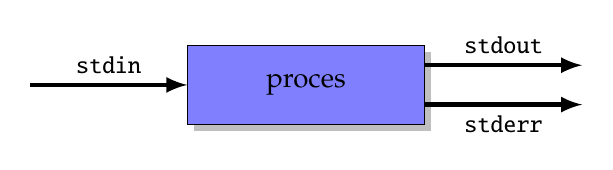
\begin{tikzpicture}
      \node[process] (process) at (0,0) {proces};
      \draw[stream] ($ (process.west) + (-2,0) $) -- (process.west) node[above,midway] {\ttfamily\small stdin};
      \draw[stream] ($ (process.east) + (0,0.25) $) -- ++(2,0) node[above,midway] {\ttfamily\small stdout};
      \draw[stream] ($ (process.east) + (0,-0.25) $) -- ++(2,0) node[below,midway] {\ttfamily\small stderr};
    \end{tikzpicture}
  \end{center}
\end{frame}

\begin{frame}
  \frametitle{Standaardstreams in Verschillende Talen}
  \begin{center}
    \begin{tabular}{llll}
      \bfseries Taal & \bfseries stdin & \bfseries stdout & \bfseries stderr \\
      \toprule
      Java & \texttt{System.in} & \texttt{System.out} & \texttt{System.err} \\
      C++ & \texttt{std::cin} & \texttt{std::cout} & \texttt{std::cerr} \\
      Python & \texttt{sys.stdin} & \texttt{sys.stdout} & \texttt{sys.stderr} \\
      C$^\sharp$ & \texttt{Console.In} & \texttt{Console.Out} & \texttt{Console.Error} \\
      Ruby & \texttt{STDIN} & \texttt{STDOUT} & \texttt{STDERR} \\
      \bottomrule
    \end{tabular}
  \end{center}
\end{frame}

\begin{frame}
  \frametitle{Standaard Streams}
  \begin{center}
    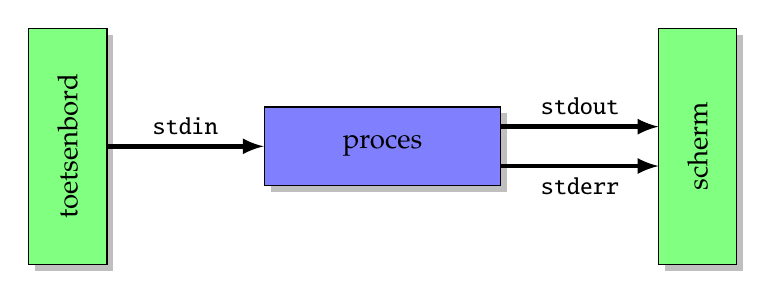
\begin{tikzpicture}
      \node[process] (process) at (0,0) {proces};
      \node[file,rotate=90] (keyboard) at (-4,0) {toetsenbord};
      \node[file,rotate=90] (screen) at (4,0) {scherm};

      \draw[stream] ($ (process.west) + (-2,0) $) -- (process.west) node[above,midway] {\ttfamily\small stdin};
      \draw[stream] ($ (process.east) + (0,0.25) $) -- ++(2,0) node[above,midway] {\ttfamily\small stdout};
      \draw[stream] ($ (process.east) + (0,-0.25) $) -- ++(2,0) node[below,midway] {\ttfamily\small stderr};
    \end{tikzpicture}
  \end{center}
  \structure{Bij opstarten proces in shell}
  \begin{itemize}
    \item stdin wordt verbonden met toetsenbord
    \item stdout en stderr worden verbonden met scherm
  \end{itemize}
\end{frame}

\begin{frame}
  \frametitle{Voorbeeld: cat}
  \begin{overprint}
    \onslide<1>
    \code[language=python,title=cat.py]{cat.py}
    \onslide<2>
    \code[language=python,title=cat.py]{cat2.py}
    \onslide<3>
    \code[language=python,title=cat.py]{cat3.py}
  \end{overprint}
  \begin{itemize}
    \item Opstarten in shell met \texttt{python cat.py}
    \item Leest stdin en schrijft naar stdout
    \item Alles wat je intypt, wordt herhaald
    \item<2-> \texttt{print} is een shortcut voor \texttt{sys.stdout.write}
    \item<2-> \texttt{input} is een shortcut voor \texttt{sys.stdin.readline()}
  \end{itemize}
\end{frame}

\begin{frame}
  \frametitle{Voorbeeld: upper}
  \code[language=python,title=upper.py,width=.95\linewidth]{upper.py}
  \begin{itemize}
    \item Opstarten in shell met \texttt{python upper.py}
    \item Herhaalt alles in uppercase
  \end{itemize}
\end{frame}

\begin{frame}
  \frametitle{Voorbeeld: filter}
  \code[language=python3,width=.9\linewidth]{filter.py}
  \begin{itemize}
    \item Opstarten in shell met \texttt{python filter.py}
    \item Herhaalt enkel lijnen die niet beginnen met \#
  \end{itemize}
\end{frame}

\begin{frame}
  \frametitle{Voorbeeld: Combinatie}
  \code[language=bash]{pipe-filter-upper.sh}
  \begin{center}
    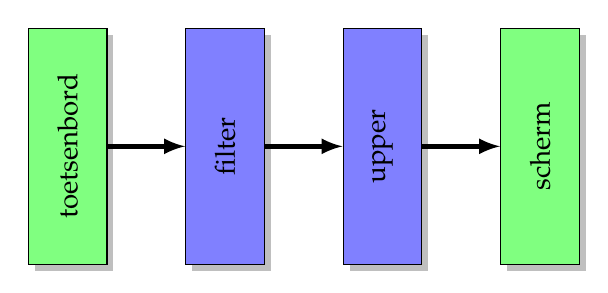
\begin{tikzpicture}[rotate=90,transform shape]
      \visible<4->{
        \node[file] (keyboard) at (0,6) {toetsenbord};
      }

      \visible<1->{
        \node[process] (filter) at (0,4) {filter};
      }
      \visible<2->{
        \node[process] (upper) at (0,2) {upper};
      }

      \visible<5->{
        \node[file] (screen) at (0,0) {scherm};
      }

      \visible<4->{
        \draw[stream] (keyboard) -- (filter);
      }

      \visible<3->{
        \draw[stream] (filter) -- (upper);
      }

      \visible<5->{
        \draw[stream] (upper) -- (screen);
      }
    \end{tikzpicture}
  \end{center}
  \begin{overprint}
    \onslide<1> \centering
    \texttt{filter} wordt opgestart
    \onslide<2> \centering
    \texttt{upper} wordt opgestart
    \onslide<3> \centering
    stdout van \texttt{filter} wordt verbonden met stdin van \texttt{upper}
    \onslide<4> \centering
    stdin van \texttt{filter} wordt verbonden met toetsenbord
    \onslide<5> \centering
    stdout van \texttt{upper} wordt verbonden met scherm
  \end{overprint}
\end{frame}

\begin{frame}
  \frametitle{Command Line Arguments}
  \begin{itemize}
    \item \texttt{filter.py} verwijdert strings beginnend met \texttt{\#}
    \item Wat als we lijnen beginnend met \texttt{//} weg willen?
    \item We kunnen een nieuw script schrijven
    \item We kunnen ook gebruik maken van parameters
  \end{itemize}
  \code[language=bash]{filter2.sh}
\end{frame}

\begin{frame}
  \frametitle{Implementatie Slimmere Filter}
  \code[language=python,font=\small]{filter2.py}
  \codeunderlinex{sysargv}
  \begin{itemize}
    \item \texttt{sys.argv} is een lijst argumenten
    \item Opgelet: het eerste argument zit in \texttt{sys.argv[1]}!
  \end{itemize}
\end{frame}

\begin{frame}
  \frametitle{Command-Line Arguments in Java}
  \code[language=java,font=\small,width=.9\linewidth]{Echo.java}
  \code[language=bash,width=.9\linewidth]{cla.sh}
\end{frame}

\begin{frame}
  \frametitle{Shell}
  \begin{center}
    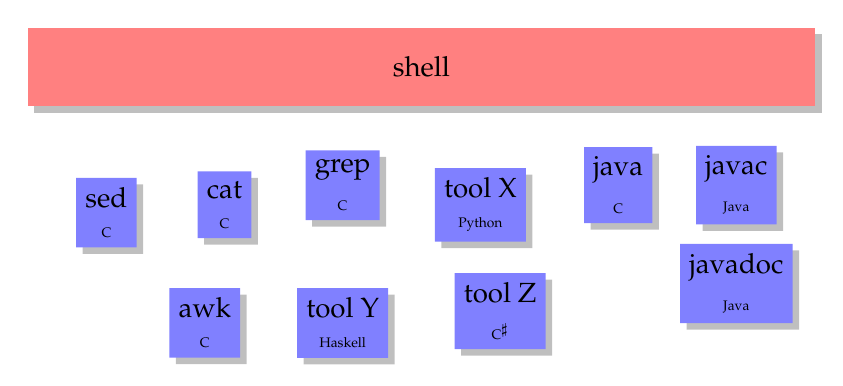
\begin{tikzpicture}[app/.style={rectangle split,rectangle split parts=2,fill=blue!50,drop shadow}]
      \node[minimum width=10cm,minimum height=1cm,fill=red!50,drop shadow] at (0,2) {shell};

      \node[app] at (-2.5,0.25) {
        cat
        \nodepart{two}
        \tiny C
      };
      \node[app] at (-4,0.15) {
        sed
        \nodepart{two}
        \tiny C
      };
      \node[app] at (-2.75,-1.25) {
        awk
        \nodepart{two}
        \tiny C
      };
      \node[app] at (-1,0.5) {
        grep
        \nodepart{two}
        \tiny C
      };
      \node[app] at (2.5,0.5) {
        java
        \nodepart{two}
        \tiny C
      };
      \node[app] at (4,0.5) {
        javac
        \nodepart{two}
        \tiny Java
      };
      \node[app] at (4,-0.75) {
        javadoc
        \nodepart{two}
        \tiny Java
      };
      \node[app] at (0.75,0.25) {
        tool X
        \nodepart{two}
        \tiny Python
      };
      \node[app] at (-1,-1.25) {
        tool Y
        \nodepart{two}
        \tiny Haskell
      };
      \node[app] at (1,-1.1) {
        tool Z
        \nodepart{two}
        \tiny C$^\sharp$
      };
    \end{tikzpicture}
  \end{center}
  \begin{itemize}
    \item Elk programma kan aanzien worden als een functie
    \item In de shell kan men deze functies oproepen
  \end{itemize}
\end{frame}



%%% Local Variables:
%%% mode: latex
%%% TeX-master: "io"
%%% End:


\end{document}



%%% Local Variables: 
%%% mode: latex
%%% TeX-master: t
%%% End: 
